\chapter{Introduction}
This report present the results from the \textit{TDT4295 Computer Design Project} course at \textit{The Norwegian University of Science and Technology} for the \textit{Camvolution} group.
In this course groups of students design and create their own computers from scratch.

The task for the Camvolution group is to create a computer optimized for performing convolution on two-dimensional data.
The processor should be able to take images and convolution kernels as input, perform the convolution, and output the convolved images.

The processor architecture should be implemented on a Xilinx FPGA, and a Silicon Labs EFM32 series microcontroller should act as an I/O processor.
The output from the processor should be displayed for demonstration purposes.
This project has a budget of 10.000 NOK.

\section{Convolution}
\begin{figure}
    \centering
    \begin{subfigure}{5cm}
        \centering
        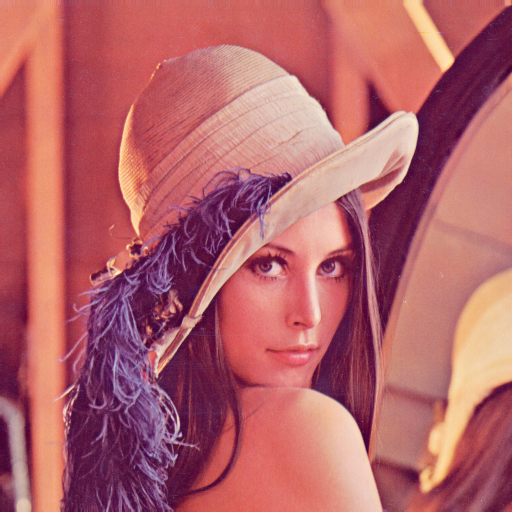
\includegraphics[width=4.5cm]{img/Lena}
        \caption{Original image}
        \label{fig:LenaOriginal}
    \end{subfigure}
    \begin{subfigure}{5cm}
        \centering
        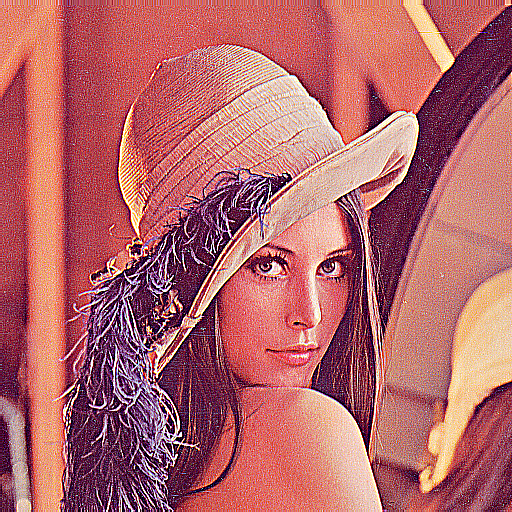
\includegraphics[width=4.5cm]{img/LenaProcessed}
        \caption{After sharpening}
    \end{subfigure}
    \caption{Lena test image}
    \label{fig:Lena}
\end{figure}
\begin{figure}
    \centering
    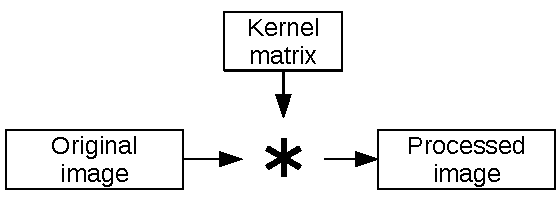
\includegraphics{img/BasicConvolution}
    \caption{Basic convolution in image processing}
    \label{fig:BasicConvolution}
\end{figure}

Convolution is a mathematical operation that can be applied to images or other signals in one or multiple dimensions.
This is commonly used by image processing software to produce blur, edge detect, sharpening filters and more.

An example of the result produced by a sharpening filter implemented with convolution can be seen in figure \ref{fig:Lena}.
The convolution itself requires two inputs, the original image and a \textit{convolution kernel matrix}.
In the case of image processing, the kernel defines what kind of filter is applied.
The inputs and outputs of convolution when used for image processing is illustrated in figure \ref{fig:BasicConvolution}.

\section{Camvolution}
The given task can be solved in multiple ways. This section presents our interpretation and the requirements for our system.

\subsection{Area of Focus}
As the task places no restrictions on what we should focus on as long as the computer performs convolution, we considered several possible areas to focus on, some inspired by the previous project reports:

\begin{enumerate}
    \item Energy efficiency
    \item Generality
    \item Performance
\end{enumerate}

In the end, the group decided to focus on performance as this would give us a more engaging demonstration, possibly with convolution performed on a live video stream.

\subsection{Requirements}
A set of goals or requirements is useful to guide the efforts in the direction of the assignment, and to ensure a demo can be held at the end of the project.

\subsubsection{Functional Requirements}
The functional requirements set for this project is listed in table \ref{tab:functional-requirements} and a more thorough descriptions follows.

\begin{table}[h]
    \centering
    \label{tab:functional-requirements}
    \begin{tabular}{lp{12cm}l}
        Name & Description & Priority \\
        \hline
        FR1 &
            The processor should do convolution on a 2 dimensional image with at least a 3x3 convolution kernel &
            High \\
        FR2 &
            The processor should have a video port to show graphical output &
            High \\
        FR3 &
            It should be able to use a camera as input &
            Medium \\
        FR4 &
            The machine should boot and operate without an external computer &
            Medium
    \end{tabular}
    \caption{Functional Requirements}
\end{table}

\paragraph{FR1}
The processor should be able to do convolution.
As the assignment states, this should be done on a 2 dimensional structure for which we have chosen an image.
Also, convolution is meaningless with a convolution kernel smaller than 3x3, thus this is also included in the requirements.

\paragraph{FR2}
It follows directly from the \nameref{subsec:assignment-text} that we must be able to display output from an application that produces graphical data.
To accomplish this, the computer is required to have a video port that can output graphics.

\paragraph{FR3}
As we decided to focus on performance, one of our goals is to be able to do convolution on a live video stream.
This requires an input stream which we have decided should come from a video camera connected to our computer.

\paragraph{FR4}
To make the demonstration a bit smoother and ensure our computer can accomplish our goals independently, we also require that the machine should be able to boot and operate without an external computer.


\subsubsection{Non-functional Requirements}

\begin{table}[h]
    \centering
    \label{tab:non-functional-requirements}
    \begin{tabular}{lp{12cm}l}
        Name & Description \\
        \hline
        NFR1 &
            The processor should be implemented on a Xilinx FPGA \\
        NFR2 &
            The processor should use Silicon Labs EFM32 microcontroller as I/O processor \\
        NFR3 &
            The cost of developing the system should not exceed a budget of 10 000 NOK \\
    \end{tabular}
    \caption{Non-functional Requirements}
\end{table}

In addition to our functional requirements, the task at hand also enforces requirements not related to the functionality of the computer produced. These are listed in table \ref{tab:non-functional-requirements}.



